\documentclass[crop,tikz,convert={outext=.svg,command=\unexpanded{pdf2svg \infile\space\outfile}},multi=false]{standalone}[2012/04/13]

\usepackage[utf8]{inputenc}
\usepackage{amsmath, amssymb}
\usepackage{pgfplots}
\usepackage{tikz}      

\usepackage{ifthen}

%-------------------------------------
% Tikz and pgf options & definitions
%-------------------------------------
\pgfplotsset{compat=1.15}
\pgfmathsetseed{1}

\usetikzlibrary{positioning}
\usetikzlibrary{shapes}
\usetikzlibrary{backgrounds, fit}
\usetikzlibrary{calc}
\usetikzlibrary{decorations.markings}
\usetikzlibrary{matrix}

\def\colorvector at (#1,#2,#3){
\coordinate (A) at (#1, #2);
\filldraw[draw=black,fill=test!!+] (A)++(0,0) rectangle ++(0.25,0.25) node (A0) {};
\filldraw[draw=black,fill=test!!+] (A)++(0.3,0) rectangle ++(0.25,0.25) node (A1) {};
\filldraw[draw=black,fill=test!!+] (A)++(0.6,0) rectangle ++(0.25,0.25) node (A2) {};
\node[right=of A2, xshift=-7.5ex, yshift=-0.75ex] {$\ldots$};
\filldraw[draw=black,fill=test!!+] (A)++(1.5,0) rectangle ++(0.25,0.25) node (A4) {};
\node[left=of A1, xshift=4.4ex, yshift=-0.75ex] (BEG\i) {$#3=[$};
\node[right=of A4, xshift=-8ex, yshift=-0.75ex] (END\i) {$]^{T}$};
}


%The matrix in numbers
%Horizontal target class
%Vertical output class
\def\myConfMat{{
{899,  50,  67, 0},  %row 1
{   0, 778, 220, 133},  %row 2
{   0,  70, 833, 1123},  %row 3
{   0,  13, 57, 953},  %row 4
}}

\def\classNames{{"$\ell_{1}$", "$\ell_{2}$", "$\ell_{3}$", "$\ell_{4}$"}} %class names. Adapt at will

\def\numClasses{4} %number of classes. Could be automatic, but you can change it for tests.

\def\myScale{1.5} % 1.5 is a good scale. Values under 1 may need smaller fonts!

\begin{document}
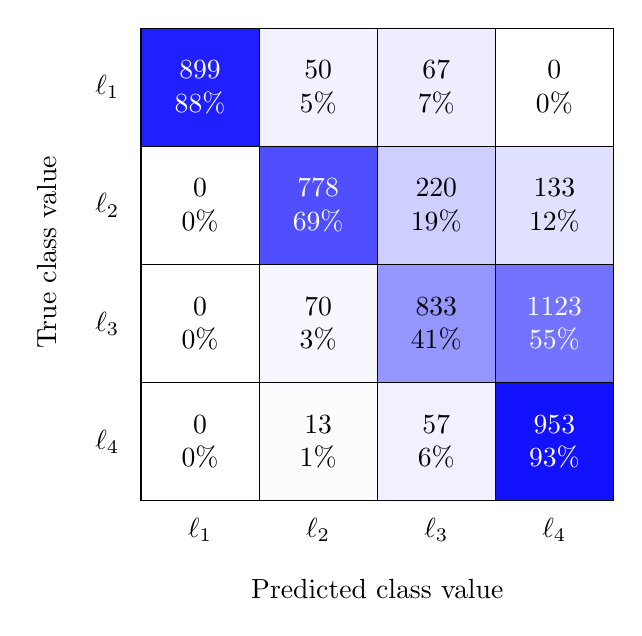
\begin{tikzpicture}[
    scale = \myScale,
    %font={\scriptsize}, %for smaller scales, even \tiny may be useful
    ]

\tikzset{vertical label/.style={rotate=90,anchor=east}}   % usable styles for below
\tikzset{diagonal label/.style={rotate=45,anchor=north east}}

\foreach \y in {1,...,\numClasses} %loop vertical starting on top
{
    % Add class name on the left
    \node [anchor=east] at (0.4,-\y) {\pgfmathparse{\classNames[\y-1]}\pgfmathresult}; 

%---- Start of automatic calculation of totSamples for the row ------------   
    \def\totSamples{0}
    \foreach \ll in {1,...,\numClasses}
    {
        \pgfmathparse{\myConfMat[\y-1][\ll-1]}   %fetch next element
        \xdef\totSamples{\totSamples+\pgfmathresult} %accumulate it with previous sum
        %must use \xdef for global effect otherwise lost in foreach loop!
    }
    \pgfmathparse{\totSamples} \xdef\totSamples{\pgfmathresult}  % put the final sum in variable
%---- End of automatic calculation of totSamples ----------------
    
    \foreach \x in {1,...,\numClasses}  %loop horizontal starting on left
    {
    
    \begin{scope}[shift={(\x,-\y)}]
        \def\mVal{\myConfMat[\y-1][\x-1]} % The value at index y,x (-1 because of zero indexing)
        \pgfmathtruncatemacro{\r}{\mVal}   %
        \pgfmathtruncatemacro{\p}{round(\r/\totSamples*100)}
        \coordinate (C) at (0,0);
        \ifthenelse{\p<50}{\def\txtcol{black}}{\def\txtcol{white}} %decide text color for contrast
        \node[
            draw,                 %draw lines
            text=\txtcol,         %text color (automatic for better contrast)
            align=center,         %align text inside cells (also for wrapping)
            fill=blue!\p,        %intensity of fill (can change base color)
            minimum size=\myScale*10mm,    %cell size to fit the scale and integer dimensions (in cm)
            inner sep=0,          %remove all inner gaps to save space in small scales
            ] (C) {\r\\\p\%};     %text to put in cell (adapt at will)
        %Now if last vertical class add its label at the bottom
        \ifthenelse{\y=\numClasses}{
        \node [] at ($(C)-(0,0.75)$) % can use vertical or diagonal label as option
        {\pgfmathparse{\classNames[\x-1]}\pgfmathresult};}{}
    \end{scope}
    }
}
%Now add x and y labels on suitable coordinates
\coordinate (yaxis) at (-0.3,0.5-\numClasses/2);  %must adapt if class labels are wider!
\coordinate (xaxis) at (0.5+\numClasses/2, -\numClasses-1.25); %id. for non horizontal labels!
\node [vertical label] at (yaxis) {True class value};
\node []               at (xaxis) {Predicted class value};
\end{tikzpicture}
\end{document}